\documentclass[a4paper]{article} 
\addtolength{\hoffset}{-2.25cm}
\addtolength{\textwidth}{4.5cm}
\addtolength{\voffset}{-3.25cm}
\addtolength{\textheight}{5cm}
\setlength{\parskip}{0pt}
\setlength{\parindent}{0in}

%----------------------------------------------------------------------------------------
%	PACKAGES AND OTHER DOCUMENT CONFIGURATIONS
%----------------------------------------------------------------------------------------

\usepackage{blindtext} % Package to generate dummy text
\usepackage{charter} % Use the Charter font
\usepackage[utf8]{inputenc} % Use UTF-8 encoding
\usepackage{microtype} % Slightly tweak font spacing for aesthetics
\usepackage[english, ngerman]{babel} % Language hyphenation and typographical rules
\usepackage{amsthm, amsmath, amssymb} % Mathematical typesetting
\usepackage{float} % Improved interface for floating objects
\usepackage[final, colorlinks = true, 
            linkcolor = black, 
            citecolor = black]{hyperref} % For hyperlinks in the PDF
\usepackage{graphicx, multicol} % Enhanced support for graphics
\usepackage{xcolor} % Driver-independent color extensions
\usepackage{marvosym, wasysym} % More symbols
\usepackage{rotating} % Rotation tools
\usepackage{censor} % Facilities for controlling restricted text
\usepackage{listings, style/lstlisting} % Environment for non-formatted code, !uses style file!
\usepackage{pseudocode} % Environment for specifying algorithms in a natural way
\usepackage{style/avm} % Environment for f-structures, !uses style file!
\usepackage{booktabs} % Enhances quality of tables
\usepackage{tikz-qtree} % Easy tree drawing tool
\tikzset{every tree node/.style={align=center,anchor=north},
         level distance=2cm} % Configuration for q-trees
\usepackage{style/btree} % Configuration for b-trees and b+-trees, !uses style file!
\usepackage[backend=biber,style=numeric,
            sorting=nyt]{biblatex} % Complete reimplementation of bibliographic facilities
\addbibresource{ecl.bib}
\usepackage{csquotes} % Context sensitive quotation facilities
\usepackage[yyyymmdd]{datetime} % Uses YEAR-MONTH-DAY format for dates
\renewcommand{\dateseparator}{-} % Sets dateseparator to '-'
\usepackage{fancyhdr} % Headers and footers
\pagestyle{fancy} % All pages have headers and footers
\fancyhead{}\renewcommand{\headrulewidth}{0pt} % Blank out the default header
\fancyfoot[L]{} % Custom footer text
\fancyfoot[C]{} % Custom footer text
\fancyfoot[R]{\thepage} % Custom footer text
\newcommand{\note}[1]{\marginpar{\scriptsize \textcolor{red}{#1}}} % Enables comments in red on margin

%----------------------------------------------------------------------------------------

\usepackage[UTF8]{ctex}
\usepackage{hyperref}
\newtheorem{theorem}{定理}
\newtheorem{example}{例}
\newtheorem{definition}{定义}
\newtheorem{lem}{引理}
\newtheorem{prof}{证明}
\usepackage{tikz-cd}
\usepackage{tikz}
\usetikzlibrary{calc,intersections,through,backgrounds}
\usepackage{tkz-euclide}

\begin{document}
%-------------------------------
%	TITLE SECTION
%-------------------------------

\fancyhead[C]{}
\hrule \medskip % Upper rule
\begin{minipage}{0.295\textwidth} 
\raggedright
\footnotesize
姓名:邓志远 \\   
 
\end{minipage}
\begin{minipage}{0.4\textwidth} 
\centering 
\large 
物理与平面几何\\ 
\normalsize 
牛顿万有引力定律的证明\\ 
\end{minipage}
\begin{minipage}{0.295\textwidth} 
\raggedleft
\today\hfill\\
\end{minipage}
\medskip\hrule 
\bigskip

\renewcommand{\contentsname}{目录}
\tableofcontents
%-------------------------------
%	CONTENTS
%-------------------------------

\section{实验事实}
最早在15世纪,丹麦科学家第谷(Tycho Brahe)穷尽一生观测得到了大量的天文数据。但是可怜的是他从正确的数据中得到了错误的结论:太阳围绕地球转,其他行星围绕太阳转。自始自终第谷相信他的第谷系统,有趣的是同时期中国明朝使用了主要依据第谷的观测结果而编制的时宪历\footnote{此内容源自维基百科\href{https://zh.wikipedia.org/wiki/第谷·布拉赫}{第谷——地心说}。但是关于为何当时中国明朝能够得到并且使用丹麦科学家第谷的数据并没有找有效记载。}。第谷作为一位科学家,是有足够历史功绩的。他最伟大的作品应当是他的学生 :开普勒(Johannes Kepler)。

\begin{theorem}
开普勒三定律:
\begin{enumerate}
    \item 行星以椭圆轨道绕太阳运行;
    \item 行星的椭圆轨道单位时间内,椭圆焦点到椭圆轨道连线扫过的面积相同,见图\ref{kepler2};
    \item 行星的公转周期的平方与长轴的立方正相关:$\frac{T^{2}}{a^{3}}=C$。
\end{enumerate}
\end{theorem}

    \begin{figure}[htp]
        \centering
        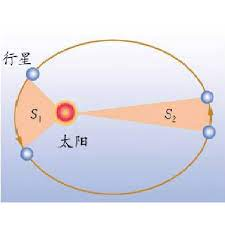
\includegraphics{kepler2.jpg}
        \caption{开普勒第二定律}
        \label{kepler2}
    \end{figure}

从他老师第谷遗留的浩渺的数据中,再加之错误方向的引领下,开普勒能够得到如此结论是伟大的。但是可惜的是他仅仅能够给出来观测结论,并不能回答“为什么会这样”。所以正如英国诗人亚历山大·蒲柏的歌颂:自然和自然的法则隐藏在黑暗之中。
上帝说:让牛顿(Sir Isaac Newton)出世吧,
于是一切豁然开朗\footnote{原文为:“Nature and nature's laws lay hid in night; God said "Let Newton be" and all was light.”}。
\section{牛顿的成果小结}
让我们给一个简洁的列表:
\begin{enumerate}
    \item 牛顿三大定律:
    \begin{enumerate}
        \item 惯性定律:在不受任何的外力或者合外力为零的情况下,物体保持静止或匀速直线运动;
        \item 相互作用:对受力物体施加力的作用后,受力物体会反过来对施力物体产生大小相等,方向相反的力;
        \item 加速度:$F=ma$。
    \end{enumerate}
    \item 万有引力定律:理论解释了开普勒定律\footnote{著名的苹果。};

    \item 动量和角动量守恒定律;
    \item 光学:反射望远镜,并完成了可见白光的光谱的观察,提出了颜色理论;
    \item 热学: 冷却定律,并给出了音速;
    \item 广为接受的历史事实,牛顿和莱布尼茨在大约同一时间创造微积分\footnote{时至今日,我们数学中沿用的解释和符号来自莱布尼茨。};牛顿证明了广义二项式定理。牛顿折线法近似函数零点,在幂级数的性质上牛顿也有重要贡献。判断一元多项式,形式幂级数的零点赋值使用的方法称之为牛顿多边形。
    \item 反假币先锋战士;
    \item 魔法炼金术士;
    \item 终究级神棍;
\end{enumerate}
牛顿的一生是毋庸置疑,无法想象的伟大,尽管他的晚年有着一些在现代看来有点滑稽的事情\footnote{内容来自维基百科\href{https://zh.wikipedia.org/wiki/艾萨克·牛顿}{艾萨克牛顿}}。
\section{万有引力定律}
众所周知,一个苹果砸到牛顿的头上,然后牛顿问:“为什么苹果会掉下来?”,他问最重要的问题是“如果有某种力让苹果掉下来,但是为什么月亮没有掉下来?”
\begin{theorem}
牛顿的万有引力定律(英语:Newton's law of universal gravitation),通称万有引力定律,定律指出,两个质点彼此之间相互吸引的作用力,是与它们的质量乘积成正比,并与它们之间的距离成平方反比\footnote{高中我们熟知的公式:$F=\frac{Gm_{1}m_{2}}{r^{2}}$(两个物体的质量为 $m_{1}$和$m_{2}$,两个物体之间的万有引力为 $F$,$r$ 为两个物体之间的距离,$G$ 为万有引力常数),准确而言牛顿并没有提出这个公式,他仅仅说明了与 $r^{2}$ 成反比。其中的万有引力常数 $G=(6.67430\pm0.00015)\times 10^{-11}m^{3}kg^{-1}s^{-2}$ 最早是由卡文迪许用“卡文迪许扭秤”测算。}。
\end{theorem}

    \begin{figure}[htp]
        \centering
        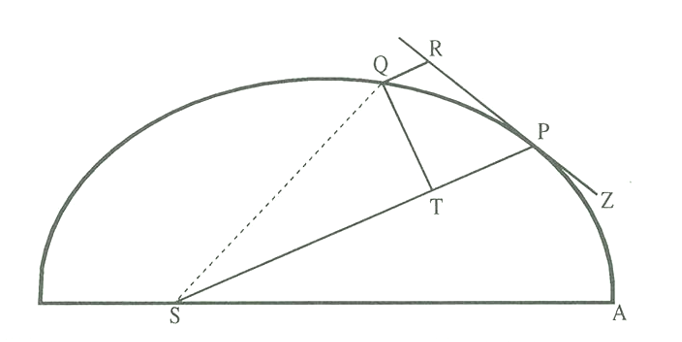
\includegraphics[scale=0.55]{newtongra.png}
        \caption{牛顿——万有引力定律}
        \label{newtongra}
    \end{figure}
    
在图\href{newtongra}中,我们给定点$P$为月亮,椭圆焦点$S$为地球。按照苹果假设,月亮应该以同样的方式进行自由落体到地球上(我们并不知道月亮和地球之间有万有引力 )。事实上,月亮在沿着轨道运动,所以自然而然的,我们可以月亮的运动看作两个运动的合成:朝向地球的自由落体,沿轨道切线的直线运动。而且当时的牛顿已经清楚的知道了自由落体运动在他的牛顿定律表述下为 $h=\frac{1}{2}at^{2}$。如图 \href{newtongra}所示,假定在极限短时间$t$内,月亮从$Q$移动到了 $P$。这种情形下,椭圆弧 $QP$ 可以近似看作线段,则月亮朝向地球方向下落的距离为 $QR$。由上述自由落体公式,可得 $a=\frac{2QR}{t^{2}}$,由牛顿加速度定律:$F=ma$,可得 $F=2m\frac{QR}{t^{2}}$。对于整个椭圆而言,均可使用三角形近似。如图\href{newtonlimit}所示,根据开普勒定律,在给定相同时间段$t$,每个以$S$为顶点,相邻节点为底的三角形面积相同,比如三角形$SFE$面积等于三角形$SED$面积。

\begin{figure}[htp]
    \centering
    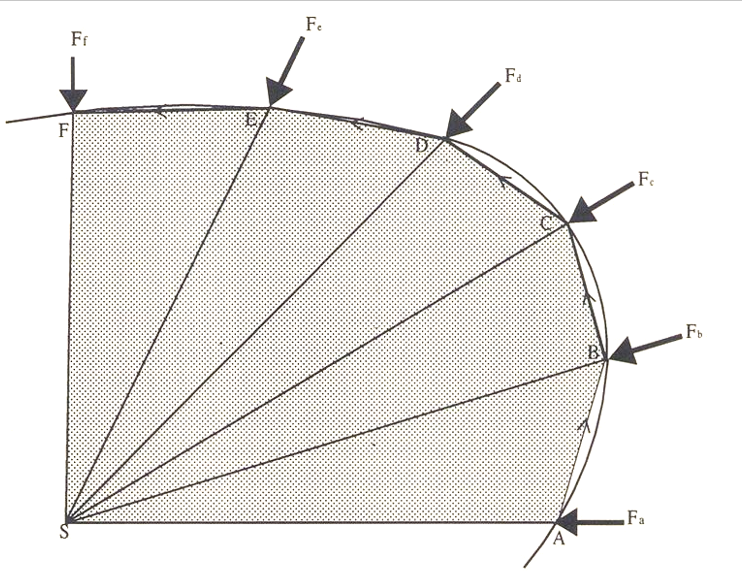
\includegraphics[scale=0.4]{newtonlimit.png}
    \caption{用多边形的极限近似椭圆}
    \label{newtonlimit}
\end{figure}
但是正如之前所说,开普勒定律是观测归纳结论,并没有严格理论解释。牛顿通过三角形全等证明了这个“单位时间内扫过的面积相等”的结论,他的证明是非常优雅的。图\href{samearea}中$CbAB$为一个平行四边形,所以三角形$BCb$与三角形$ABb$面积相等。剩余部分$\Delta SbC$与 $\Delta SAb$面积也相等,因为同底等高。


\begin{figure}[htp]
    \centering
    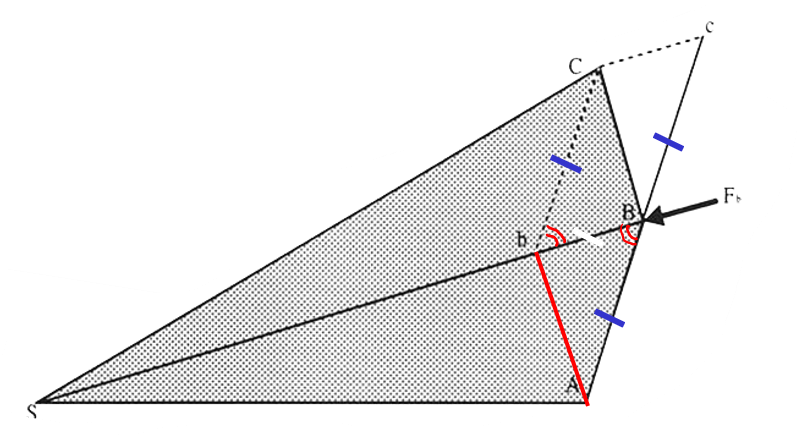
\includegraphics[scale=0.5]{samearea.png}
    \caption{三角形全等}
    \label{samearea}
\end{figure}

总结一下,上述所得到的结论:相同时间内,月亮($P$点)与地球($S$点/焦点 )连线扫过的面积相同。换而言之,每个单位时间对应的每个三角形面积相同,即时间与扫过的面积正相关:$t\propto (\frac{1}{2}QT\times SP)$。将这个正比关系代入,得到
\begin{equation*}
    F=ma=2m\frac{QR}{t^{2}}\propto\frac{QR}{QT^{2}\times SP^{2}}=\frac{QR}{QT^{2}}\times \frac{1}{SP^{2}}.
\end{equation*}

目标是证明:$F\propto \frac{1}{SP^{2}}$。所以下一步就是要证明:
\begin{lem}
若 $Q$ 在 $P$ 的无穷小领域中,$\frac{QR}{QT^{2}}$为$2SL$ (短轴长),即常数。

\begin{figure}[htp]
    \centering
    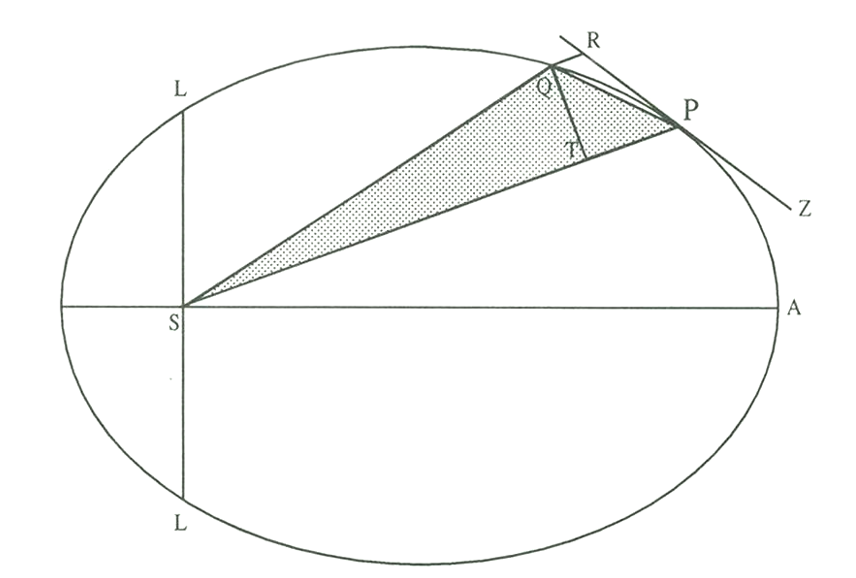
\includegraphics[scale=0.5]{ellptic.png}
    \caption{引理}
    \label{ellptic}
\end{figure}
\end{lem}
\begin{prof}
这玩意留作高中生的作业题吧。
\end{prof}
\end{document}
